\chapter{Návrh zařízení}

Tato kapitola se bude zabývat návrhem hardwaru celého zařízení. Jedním z hlavních požadavků je nízká spotřeba, kterou bude třeba zohlednit při vybírání použitých senzorů, řídícího mikroprocesoru, komunikačního modulu a ostatních obvodových komponent. 

\section{Výběr senzorů}
Celé zařízení bude schopno měřit koncentraci prachových částic, koncentraci oxidu uhelnatého, intenzitu osvětlení, intenzitu UV záření, teplotu, atmosférický tlak a relativní vlhkost. V následujících částech tedy bude popsán výběr z dostupných senzorů.

\subsection{Senzor koncentrace prachových částic}

Na trhu je dostupných hned několik senzorů na měření koncentrace prachových částic. Jak již bylo zmíněno v teoretickém úvodu, budu vybírat senzor, který tuto koncentraci určuje na zákkladě osvícení daného vzorku vzduchu a následně měření odraženého světla. Nyní vyvstává otázka, jestli zvolit senzor, který bude vzorek vzduchu vhánět do měřícího prostoru nuceně pomocí ventilátoru nebo jen za využití stoupání teplého vzduchu nahoru. V tabulce \ref{tab_DustSensors} jsou uvedeny senzory, které jsou relativně cenově přijatelné, a~daly by se pro neprofesionální měření využít.

\newcommand{\ugcm}{\micro\gram\per\cubic\meter} % define new command used in '\SI' -> micro gram per cubic meter

\begin{table}[h]
    \centering
    \begin{tabular}{c|cccc}
    \textbf{Název}           & \textbf{Rozlišení}                & \textbf{Přesnost}                              & \textbf{Proud}                           & \textbf{Čas čtení}                \\ \hline
    \multirow{2}{*}{PMS5003} & \multirow{2}{*}{\SI{1}{\ugcm}}    & $0-100$\SI{}{\ugcm}:$\pm$\SI{10}{\micro\gram}  & \multirow{2}{*}{\SI{100}{\milli\ampere}} & \multirow{2}{*}{\SI{10}{\second}} \\
                             &                                   & $100-500$\SI{}{\ugcm}:$\pm$\SI{10}{\percent}   &                                          &                                   \\ \hline
    \multirow{2}{*}{PM1003}  & \multirow{2}{*}{\SI{1}{\ugcm}}    & $0-100$\SI{}{\ugcm}:$\pm$\SI{30}{\micro\gram}  & \multirow{2}{*}{\SI{90}{\milli\ampere}}  & \multirow{2}{*}{\SI{30}{\second}} \\
                             &                                   & $100-500$\SI{}{\ugcm}:$\pm$\SI{30}{\percent}   &                                          &                                   \\ \hline
    \multirow{2}{*}{PM1006}  & \multirow{2}{*}{neuvedeno}        & $0-100$\SI{}{\ugcm}:$\pm$\SI{20}{\micro\gram}  & \multirow{2}{*}{\SI{30}{\milli\ampere}}  & \multirow{2}{*}{\SI{8}{\second}}  \\
                             &                                   & $100-500$\SI{}{\ugcm}:$\pm$\SI{20}{\percent}   &                                          &                                   \\ \hline
    GP2Y1010AU0F             & \SI{0,5}{\volt}$/$\SI{100}{\ugcm} & záleží na ADC                                  & \SI{20}{\milli\ampere}                   & \SI{1}{\second}                           
    \end{tabular}
    \caption{Porovnání vybraných parametrů senzorů koncentrace prachových částic}
    \label{tab_DustSensors}
\end{table}

Po pečlivém prostudování jednotlivých parametrů jsem zvolil senzor PMS5003 od firmy PLANTOWER. Důležitým aspektem při výběru byla také cena tohoto senzoru, v době vypracovávání této práce jej šlo pořídit za zhruba 350~Kč. Dalším důležitým parametrem byla spotřeba proudu v aktivním stavu, na první pohled se může zdát, že oproti všem senzorům má spotřebu nejvyšší. Oproti PM1003 má však třetinový čas potřebný k získání měřených dat, takže spotřebovává sice vyšší proud, ale po kratší časový úsek. PM1006 má spotřebu proudu zhruba třetinovou, ale vzorek měřeného vzudchu se do měřícího prostoru dostává pomocí sálání a tak je nutné zajistit konstrukčně dostatečně a správně dimenzované průduchy a také konstantní polohu a hlavně náklon senzoru, což by mohlo být v praxi téměř nemožné, pokud má být zařízení používáno také ve volném prostranství. Poslední ze senzorů v tabulce \ref{tab_DustSensors} má zdánlivě nejlepší výsledky. Bohužel se jedná pouze o měřící modul samotný, který neobsahuje žádný ventilátor ani řídící logiku, je tedy třeba tyto věci zapojit a konstrukčně vyřešit. Nejjednodušší na obvodové zapojení, a i z hlediska parametrů přesnosti nejlepší, se tak jeví již zmíněný senzor PMS5003.

\begin{figure}
    \centering
    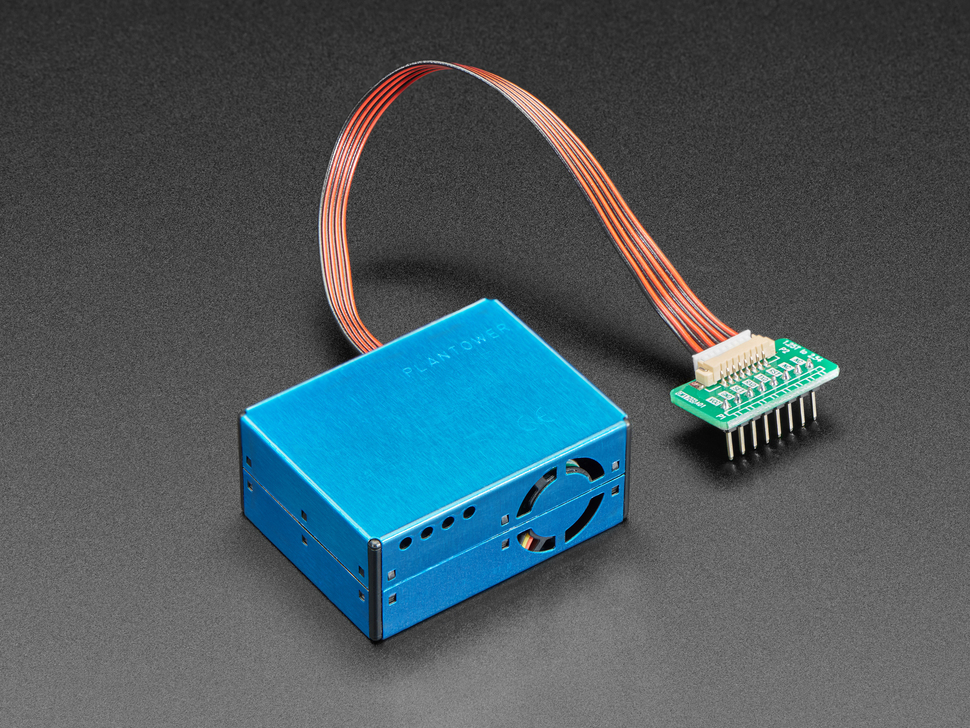
\includegraphics[width=0.7\textwidth]{obrazky/PMS5003.jpg}
    \caption{Senzor pro měření koncentrace prachových částic PMS5003. \cite{dat_PMS5003}}
    \label{fig_PMS5003}
\end{figure}

\subsection{Senzor oxidu uhelnatého}

